% !TeX root = ../main.tex

\chapter{Experimental Setup}\label{chapter:experimental-setup}

We briefly document the hardware, software stack, and facilities enabling reproducible experiments.

\section{Hardware}
- Airframe: X-wing aerodynamic surface-enhanced quadrotor.
- Propulsion: motors, ESCs, props; thrust-to-weight and voltage.
- Avionics: Flight Controller (Betaflight/Agilicious/Pilot), Jetson companion, IMU, telemetry.

\subsection{Bill of Materials (BOM)}
Table~\ref{tab:bom} lists the main components. 

\begin{table}[htbp]
	\caption[Bill of materials]{Bill of materials for the platform.}
	\label{tab:bom}
	\centering
	\setlength{\tabcolsep}{6pt}% tighter columns
	\renewcommand{\arraystretch}{1.1}% a bit more row height
	\begin{tabularx}{\textwidth}{ll>{\raggedright\arraybackslash}X}
		Category & Component & Model / Key specs \\
		\midrule
	Airframe & Frame & X-wing center frame with motor arms and wing mounts \\
	Airframe & Wings & Four fixed wings (each 450\,×\,250\,mm; NACA 15 airfoil), orthogonal layout ($90^{\circ}$ between adjacent wings); skins: Bambu Lab PLA Aero; spars: 10\,mm OD carbon tubes; total projected horizontal area $S\approx 0.318$\,m$^2$ \\
		Propulsion & Motor ($\times$4) & T-MOTORHOBBY VELOX V2808 \\
		Propulsion & Propeller ($\times$4) & HQProp 7\,×\,3.5\,×\,3 Racing Prop, 3-blade, 7" (Light Grey) \\
		Avionics & FC+ESC Stack & Kakute H7 v1.5 Stack (Flight Controller + 4-in-1 ESC) \\
		Wiring & Motor power & 12\,AWG wire (FC/ESC to motors) \\
		Power & Battery ($\times$2, parallel) & Tattu R-Line V5.0 LiPo, 6S, 1400\,mAh, 150C, XT60; effective 6S, 2800\,mAh (parallel) \\
		Companion & NVIDIA Jetson Orin & Orin Nano 8GB (specify exact variant), CUDA 12, 8GB LPDDR5; JetPack~6 (Ubuntu 22.04) \\
		Companion power & Battery & Tattu R-Line Version 3.0, 1800\,mAh, 4S, 14.8\,V, 120C, XT60 (via buck regulator to Jetson input) \\
		Motion capture & Vicon markers & Four 2\,cm markers arranged in an asymmetric constellation to prevent rotational ambiguity in rigid-body recognition \\
		\bottomrule
	\end{tabularx}
\end{table}

\section{Software}
- Estimation and control pipeline on FC/companion; logging.
- Vicon motion capture integration for ground truth and state feedback.

\section{Facilities}
- Flight arena for agility tests (3g circles), AIDA hall for efficiency trials.

\begin{figure}[htbp]
	\centering
	% Save the image as figures/aida_hall.jpg (download from the credited source below).
	\IfFileExists{figures/aida_hall.jpg}{%
		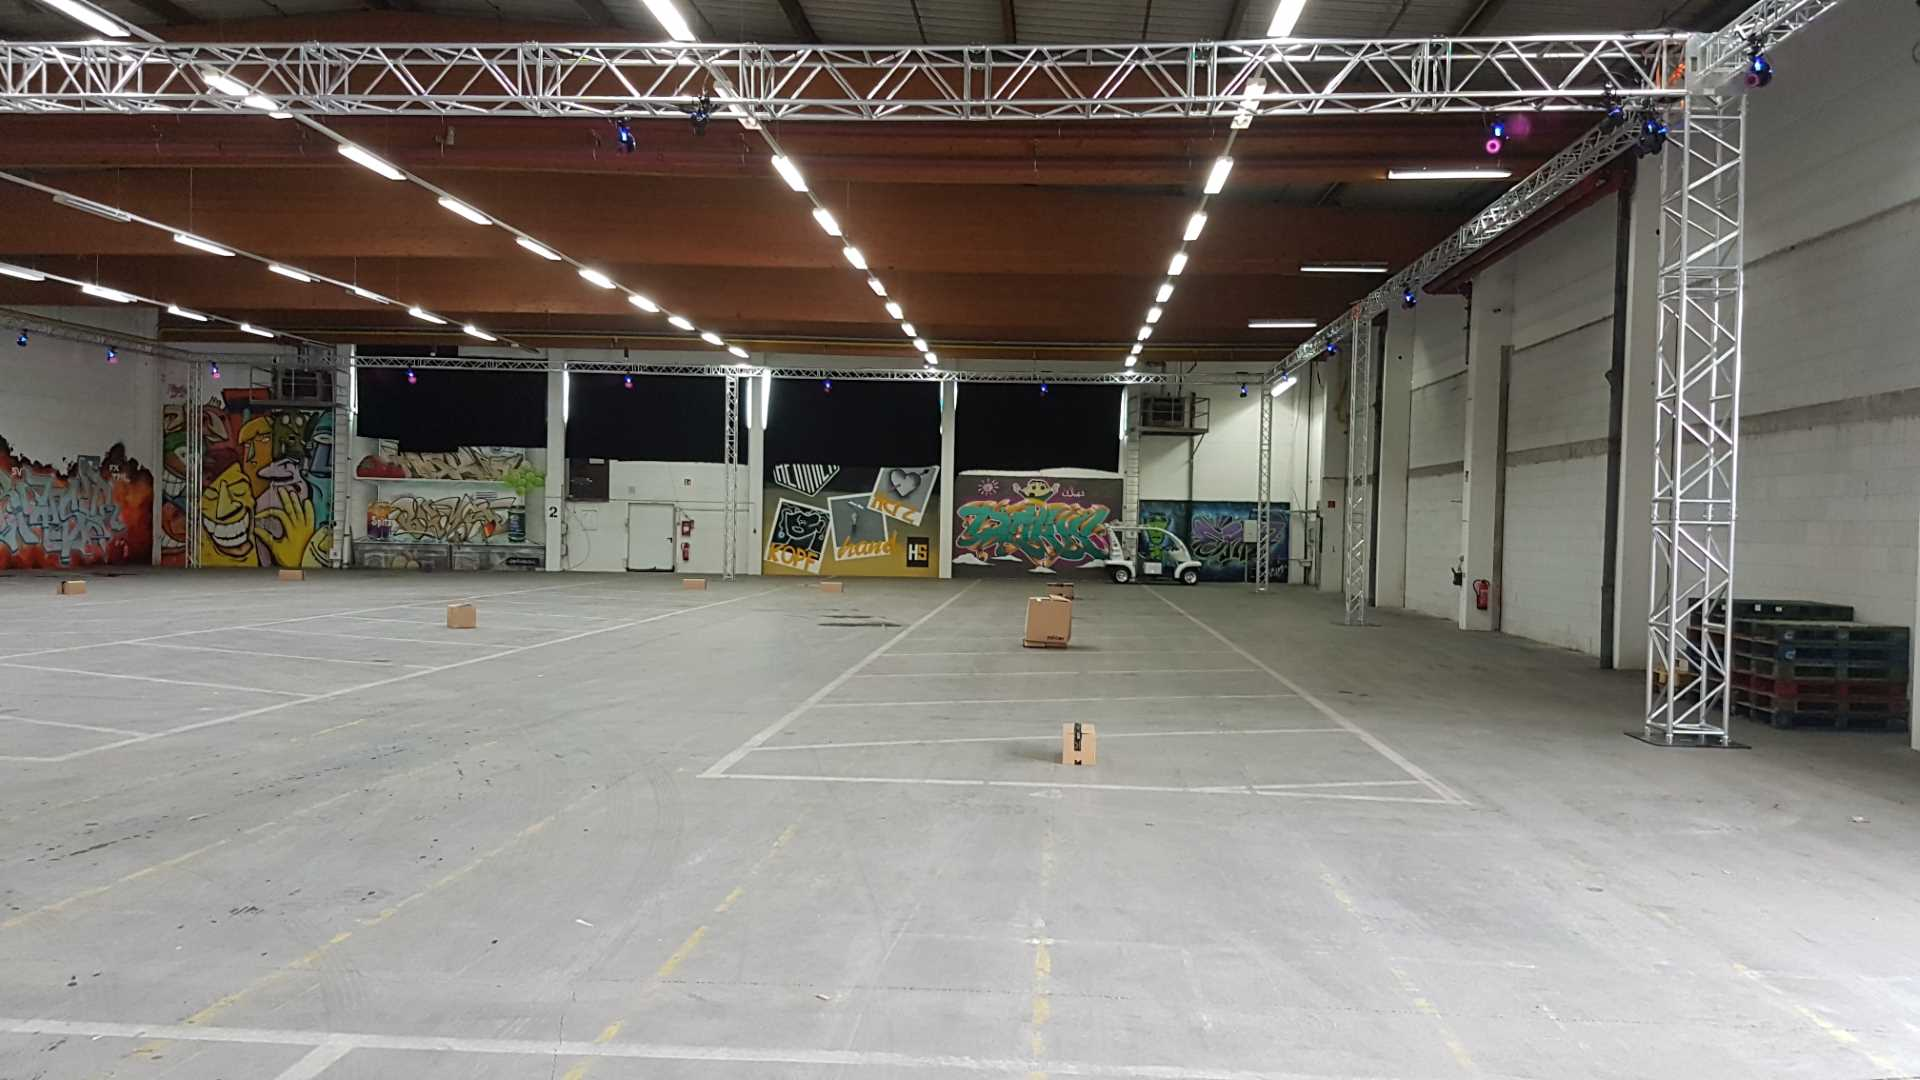
\includegraphics[width=\linewidth]{figures/aida_hall.jpg}%
	}{%
		\fbox{\parbox{0.95\linewidth}{AIDA Hall photo placeholder. Save the image to \texttt{figures/aida_hall.jpg}.}}%
	}
		\caption[AIDA Hall test facility]{AIDA Hall test facility used for efficiency trials (image credit: \textcite{AIDAHallPhoto2024}).}
	\label{fig:aida-hall}
\end{figure}
